\section{ハイパスフィルタによる画像処理}

\autoref{code:high_pass}に,画像に対してハイパスフィルタを行う$\mathsf{high\_pass\_img}()$関数を示す.
\autoref{code:high_pass}では,入力された画像から離散フーリエ変換を用いて周波数成分を抽出し,
$x, y$それぞれのカットオフ周波数より低い周波数領域に0を代入したのちに離散フーリエ逆変換
を用いて画像へと復元する.ただし,処理時間の都合上,離散フーリエ変換,逆変換はNumPy
ライブラリにて実装されている高速フーリエ変換を用いる.
\lstinputlisting[caption=画像へのハイパスフィルタを行う$\mathsf{high\_pass\_img}()$関数, label={code:high_pass}]{script/show_high_pass.py}

\autoref{fig:high_input}に入力画像,
\autoref{fig:high_pass_dft}に\autoref{fig:dft_high}に対してハイパスフィルタで
処理した後の周波数成分,
\autoref{fig:high_pass_idft}に復元した出力画像を示す.
\autoref{fig:high_pass_idft}より,画像内の顔の輪郭や髪の毛などといったよなピクセル間の
温度差の激しい部分,すなわちエッジが抽出できており,
逆に帽子の模様や鏡の縁のようなピクセル間の温度差が類似している部分が除去されている.
このことから,画像データに対してハイパスフィルタを用いることにより
画像のエッジ抽出として活用することができる.

\iffigure
\begin{figure}[h]
  \centering
  \begin{minipage}{.25\hsize}
    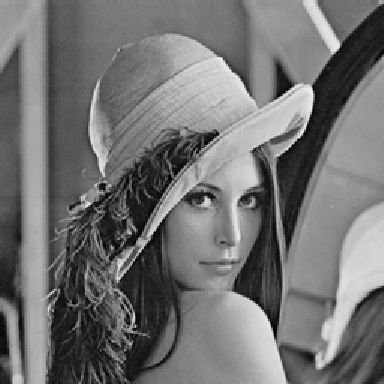
\includegraphics[clip, width=\textwidth]{figure/Lenna.pdf}
    \caption{入力画像}
    \label{fig:high_input}
  \end{minipage}
  \begin{minipage}{.25\hsize}
    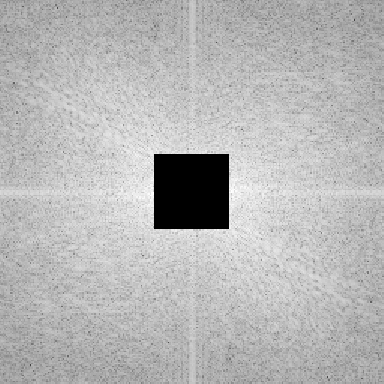
\includegraphics[clip, width=\textwidth]{figure/high_pass_dft_2d.pdf}
    \caption{ハイパスフィルタによる抽出}
    \label{fig:high_pass_dft}
  \end{minipage}
  \begin{minipage}{.25\hsize}
    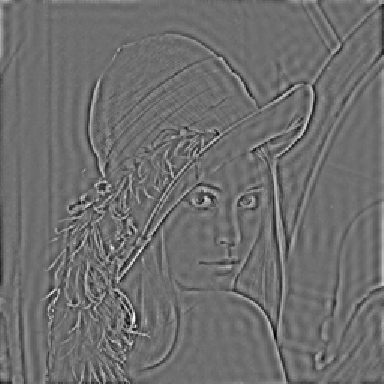
\includegraphics[clip, width=\textwidth]{figure/high_pass_idft_2d.pdf}
    \caption{処理後の画像}
    \label{fig:high_pass_idft}
  \end{minipage}
\end{figure}
\fi
